\documentclass[final]{beamer}

% ====================
% Packages
% ====================
\usepackage{amsfonts}
\usepackage[T1]{fontenc}
\usepackage{lmodern}
\usepackage[size=custom,width=30,height=48,scale=1.0]{beamerposter}
\geometry{paperwidth=30in,paperheight=48in}
\usetheme{gemini}
\usecolortheme{ucf}
\usepackage{graphicx}
\usepackage{booktabs}
\usepackage{tikz}
\usepackage{pgfplots}
\pgfplotsset{compat=1.17}

% ====================
% Lengths
% ====================
\newlength{\sepwidth}
\newlength{\colwidth}
\setlength{\sepwidth}{0.025\paperwidth}
\setlength{\colwidth}{0.3\paperwidth}

\newcommand{\separatorcolumn}{\begin{column}{\sepwidth}\end{column}}

% ====================
% Title
% ====================
\title{\textbf{YOLO Object Detection: Challenges and Evolution}}
\author{Tausif Diwan, Jitendra.V.Tembhurne}
\institute[IIITN]{Indian Institute of Information Technology, Nagpur}

% ====================
% Footer (optional)
% ====================
\footercontent{
  \href{https://iiitn.ac.in}{https://iiitn.ac.in} \hfill
  October 2023 \hfill
  \href{mailto:tdiwan@iiitn.ac.in}{tdiwan@iiitn.ac.in}
}

\begin{document}
\begin{frame}[t]
\begin{columns}[t]
\separatorcolumn

\begin{column}{\colwidth}
  \begin{block}{Abstract}
    YOLO (You Only Look Once) is a pioneering single-stage object detection algorithm that has transformed the landscape of computer vision by offering real-time detection with significantly faster inference compared to traditional multi-stage detectors like Faster R-CNN. YOLO frames the detection task as a regression problem, allowing it to predict bounding boxes and class probabilities in a single evaluation of the entire image. Since its introduction, YOLO has undergone multiple iterations—YOLOv1, YOLOv2, YOLOv3, and YOLOv4—each refining detection accuracy, speed, and the handling of small objects. YOLOv4, in particular, incorporates advanced techniques like Cross-Stage Partial Networks (CSPNet), Spatial Pyramid Pooling (SPP), and Mosaic augmentation, further improving performance while maintaining low latency.
Despite these advancements, YOLO faces challenges such as detecting small and overlapping objects and performing under conditions of image degradation due to noise, blur, or occlusion. Addressing these issues, ongoing research has focused on enhancing the model’s robustness through multi-scale feature fusion and improved loss functions. This poster outlines YOLO’s evolution, the architectural enhancements in each version, and presents results illustrating its performance across varied conditions. We also highlight future directions, such as integrating attention mechanisms to improve YOLO’s effectiveness in complex real-world scenarios.
  \end{block}
  
  \begin{block}{Introduction}
    YOLO (You Only Look Once) has gained widespread recognition for its speed and efficiency, making it ideal for real-time object detection tasks such as autonomous driving, video surveillance, and robotics. Unlike traditional multi-stage detection methods like Faster R-CNN, which rely on separate processes for region proposals, feature extraction, and classification, YOLO reframes the object detection task as a single regression problem. By dividing the input image into a grid and predicting bounding boxes and class probabilities directly from the entire image in a single forward pass, YOLO eliminates the need for region proposal stages, significantly speeding up the detection process. This innovation allows YOLO to achieve real-time performance with minimal latency. Over the years, YOLO has evolved from its initial version (YOLOv1) to more advanced iterations like YOLOv4, each improving upon accuracy, handling of smaller objects, and inference speed. These advancements have made YOLO highly adaptable to diverse real-world applications, though it continues to face challenges such as maintaining performance in degraded image conditions like blur, noise, and occlusion.
  \end{block}

  \begin{figure}
    \centering
    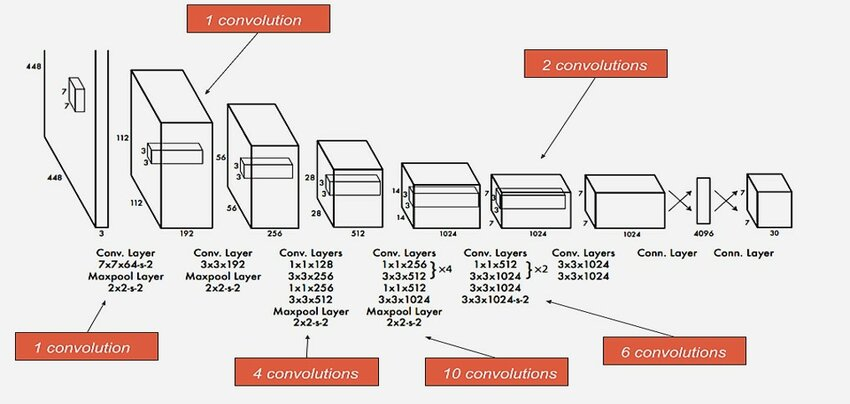
\includegraphics[width=0.95\textwidth]{logos/yolo_architecture.png}
    \caption{YOLO architecture overview}
    \label{fig:arch}
  \end{figure}

\begin{block}{Challenges in Object Detection}
    Despite its achievements, YOLO faces several persistent challenges that impact its performance in real-world scenarios. Key challenges include:

    \begin{itemize}
      \item **Multi-scale training:** YOLO's fixed grid structure limits its ability to effectively detect objects of varying sizes. This necessitates training with images that cover a wide range of scales to improve accuracy across small, medium, and large objects. If smaller objects are underrepresented, detection performance can significantly decline.

      \item **Handling small and overlapping objects:** Small objects often occupy only a few pixels in feature maps, making accurate detection difficult. Additionally, overlapping objects can create confusion, leading to incorrect predictions. YOLO's single-stage architecture may struggle with these challenges, requiring advanced techniques to differentiate overlapping entities.

      \item **Dealing with low-quality and degraded images:** Environmental factors like motion blur, noise, and occlusion can degrade image quality, hindering YOLO’s effectiveness. These issues can obscure important features necessary for detection, highlighting the need for improvements that bolster the model’s robustness against real-world conditions \cite{6}.
    \end{itemize}

    These challenges emphasize the need for ongoing research to enhance YOLO’s capabilities and ensure its reliability in diverse practical applications.
\end{block}



\end{column}

\separatorcolumn

\begin{column}{\colwidth}

\begin{block}{Key Improvements in YOLO Versions}
    YOLO has evolved through several versions, each introducing enhancements to address the limitations of its predecessors:

    \begin{itemize}
      \item **YOLOv1:** The initial version emphasized speed and real-time detection by processing the entire image in one pass. However, it struggled with recall rates and localization accuracy, especially for smaller objects, due to its coarse grid structure, which often led to missed detections.

      \item **YOLOv2:** This version introduced anchor boxes, enabling better handling of objects of varying sizes. The use of batch normalization stabilized training, while Darknet-19 as the backbone architecture improved feature extraction capabilities, allowing YOLOv2 to perform better in multi-class detection tasks.

      \item **YOLOv3:** YOLOv3 enhanced small object detection by incorporating **feature pyramids**, which leveraged multiple scales for better accuracy. The introduction of the Darknet-53 backbone with residual connections improved gradient flow, while logistic regression for class predictions enhanced its handling of overlapping objects.

      \item **YOLOv4:** The latest version introduced several optimizations, including **CSPNet** for improved gradient flow and reduced computation, and **Mosaic data augmentation** to enhance training diversity. Additionally, **Spatial Pyramid Pooling (SPP)** improved the model's ability to capture objects at different scales without increasing inference time, leading to significant gains in accuracy while maintaining fast processing speeds.

    \end{itemize}

    The continuous refinement of YOLO across these versions showcases its adaptability and relevance in the rapidly evolving field of computer vision, effectively addressing key limitations and enhancing its capabilities for real-world applications.
\end{block}



\begin{block}{Experimental Setup}
    The experiments were conducted using popular datasets, specifically **MS COCO** (Microsoft Common Objects in Context) and **PASCAL VOC** (Visual Object Classes), which are widely used benchmarks for evaluating object detection algorithms. These datasets provide diverse scenarios with a rich variety of object classes, backgrounds, and environmental conditions, making them ideal for training and testing YOLO's capabilities.

    To thoroughly evaluate the performance of YOLO, we analyzed its robustness under various image degradation conditions that simulate real-world challenges, including:

    \begin{itemize}
      \item **Blur:** This condition was simulated to replicate effects caused by camera motion or poor focus, which can obscure object details and hinder accurate detection.
      \item **Noise:** Random variations in pixel values were introduced to mimic low-light conditions or sensor noise, which often complicates the detection process by reducing image clarity.
      \item **Rotation:** We tested the model’s ability to detect objects at different orientations, assessing its robustness to variations in object alignment and perspective that occur in practical scenarios.
      \item **Cropping:** This condition assessed the model's performance when parts of objects are obscured or missing, simulating real-world situations where objects may be partially visible due to occlusion or framing.
    \end{itemize}

    The training and evaluation processes were executed on high-performance GPUs, allowing for efficient computation and the handling of large datasets. Images were processed at varying resolutions to determine the model’s adaptability and performance across different settings and to understand how resolution impacts detection accuracy. This comprehensive setup provides insights into YOLO's strengths and weaknesses under challenging conditions, informing future improvements and refinements to the algorithm.
\end{block}

  
\end{column}

\separatorcolumn

\begin{column}{\colwidth}
    \begin{block}{Results and Discussion}
    The model’s performance varied significantly with the type of image degradation applied during testing. The findings from our experiments indicate the following:

    \begin{itemize}
      \item **Blur:** This condition resulted in an average precision decrease of 2.06%. This modest decline highlights the critical need for clarity in images, as blurriness can obscure important object details, leading to inaccuracies in detection. The model's ability to recognize features diminishes when images lack sharpness, emphasizing the importance of employing effective stabilization and focus techniques in real-world applications.

      \item **Noise:** The introduction of noise to the images led to a more substantial drop in performance, with average precision lowered by 12.01%. This significant decline suggests that noise, particularly in low-light conditions, can severely impact the model's capability to accurately identify and classify objects. It points to the necessity for incorporating robust noise reduction techniques or advanced preprocessing methods to mitigate the effects of noise and improve detection accuracy.

      \item **Rotation:** Accuracy diminished by 24.23% under rotated conditions, underscoring the challenges posed by non-standard object orientations. The model's difficulty in recognizing objects at various angles suggests that additional strategies, such as augmenting the training dataset with rotated images, could enhance the model's robustness against orientation variations and improve its generalization capabilities in practical scenarios.
    \end{itemize}

    Importantly, training the model on datasets that include a variety of degradation conditions has shown to improve robustness. Exposure to challenging scenarios during the training phase equips the model with the necessary features to handle similar difficulties during inference. This finding demonstrates the value of data augmentation and diverse training methodologies in developing resilient object detection models that can perform reliably in real-world environments \cite{7}.
  \end{block}

  \begin{figure}
    \centering
    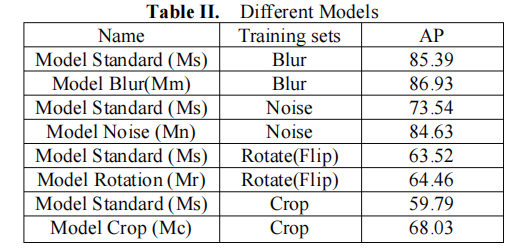
\includegraphics[width=0.95\textwidth]{logos/res_poster.png}
    \caption{Model accuracy under different degradations}
    \label{fig:results}
  \end{figure}
  
 \begin{block}{Conclusions}
    In conclusion, YOLO (You Only Look Once) remains one of the most effective object detection algorithms in the field of computer vision, primarily due to its exceptional speed and efficiency. Its single-stage architecture allows for real-time processing, making it particularly suitable for applications in areas such as autonomous driving, video surveillance, and robotics. The ability to predict bounding boxes and class probabilities in a single evaluation significantly reduces latency, enabling rapid decision-making in critical situations.

    However, despite these advantages, the model’s performance in scenarios involving degraded images—such as those affected by blur, noise, or occlusion—necessitates further optimization and advancements. The challenges associated with detecting small and overlapping objects also remain a concern, as these scenarios can lead to decreased accuracy and reliability in practical applications. 

    Future work will focus on developing innovative techniques to enhance YOLO's capability to detect small objects, which is crucial for applications that require high precision, such as medical imaging or industrial inspections. Additionally, improving performance in real-time applications that encounter poor-quality images is essential for broadening the algorithm's usability across diverse environments. 

    Continuous research and innovation in this area will ensure that YOLO maintains its relevance and utility in practical applications. By addressing these challenges, future iterations of YOLO could achieve even greater robustness and adaptability, reinforcing its position as a leading solution in the evolving landscape of object detection technologies.
\end{block}

  
\end{column}

\separatorcolumn
\end{columns}
\end{frame}
\end{document}
